%!TEX root = Main.tex

\section{Simulation}

We analyze the network with two types of nodes.
Figure \ref{fig: nodes locations} shows the locations of 50 nodes, among which 4 are from type I and the rest 46 are from type II.
The first type of nodes (type I) are equispaced points on $x=0.5$ and $0.8\leq y\leq 5.2$.
The second type of nodes (type II) are generated uniformly in $[0,1]\times[0,6]$. 
\\
\begin{figure}[htbp]
\begin{subfigure}{.25\textwidth}
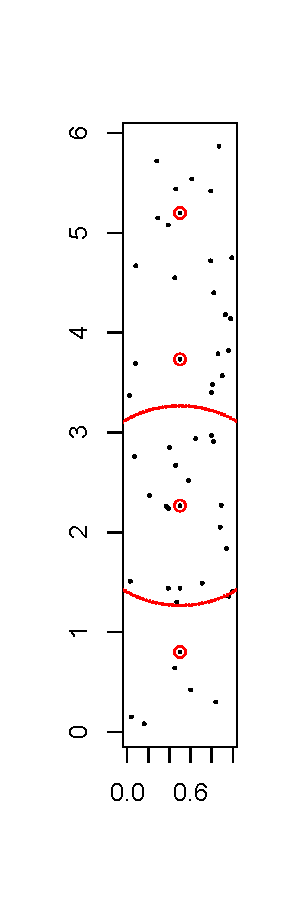
\includegraphics[width=\linewidth]{../simulation/plots/nodes_1_108}
\caption{}
\label{fig: nodes locations}
\end{subfigure}
\begin{minipage}{.74\textwidth}
\begin{subfigure}{\textwidth}
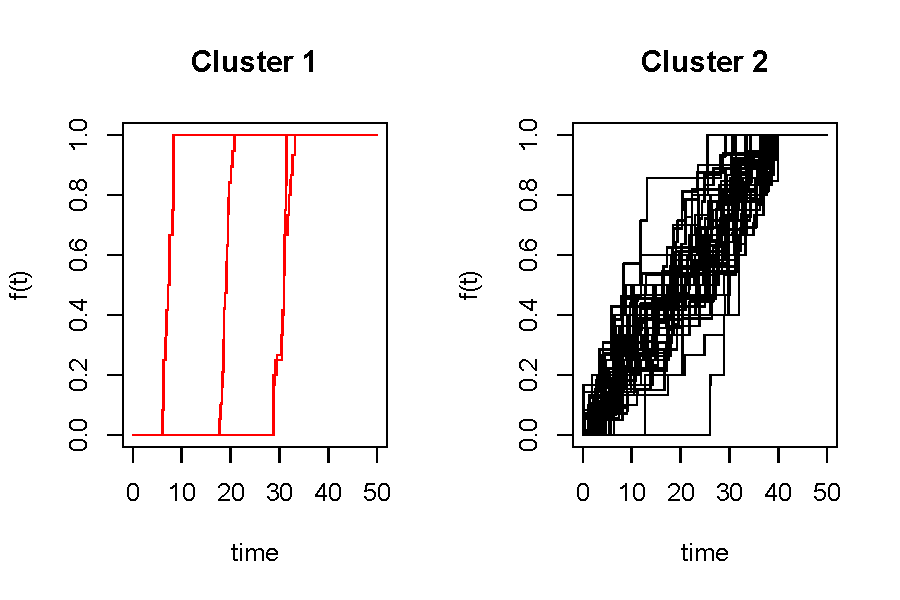
\includegraphics[width=\linewidth]{../simulation/plots/f_list_1_108}
\caption{}
\label{fig: original curves}
\end{subfigure}
\begin{subfigure}{\textwidth}
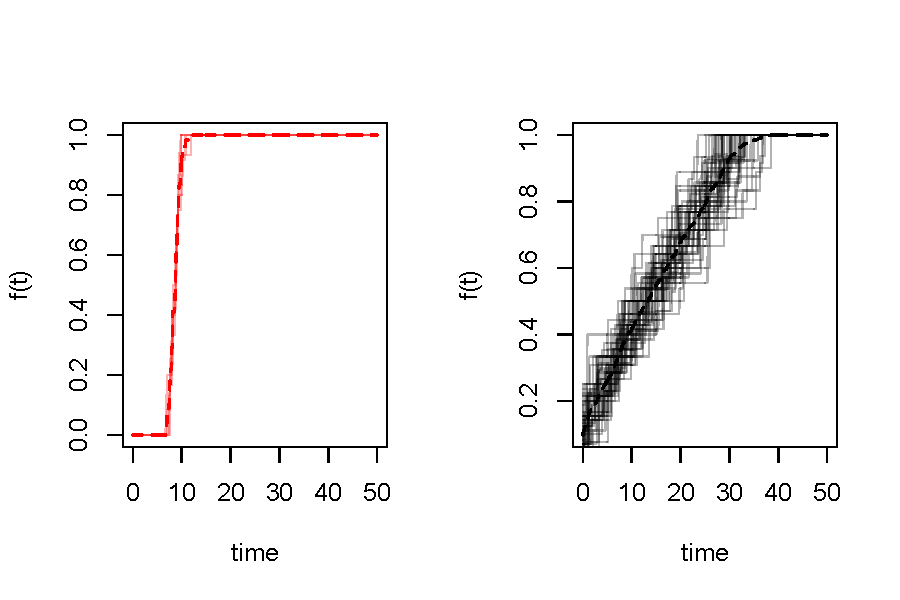
\includegraphics[width=\linewidth]{../simulation/plots/clus_results_1_108}
\caption{}
\label{fig: aligned curves}
\end{subfigure}
\end{minipage}
\caption{(a): Locations of nodes. Each black dot represents a node, the four type I nodes are marked as red. The dotted circle explains the reachable area of the second type I node. (b): Original empirical distribution functions. The red curves correspond to type I nodes, and the black curves correspond to type II nodes. (c): Clustering result. Each subplot includes the shifted distribution functions of the nodes belonging to that cluster. The mean curves are plotted by dashed lines. }
\end{figure}

The network is developed during time period $[0,50]$.
Two nodes are connected if the distance between them is less than $1$.
The connecting time between two type II nodes is generated from uniform distribution $U(0,40)$.
For the pair of nodes with one from type I and the other from type II, the connecting time is distributed as $N(5+\tau,1)$, where $\tau$ is the time delay caused by the type I node and is generated randomly from $U(0,30)$.

Figure \ref{fig: original curves} shows the empirical distribution function of the connecting time of each node.
Figure \ref{fig: aligned curves} shows clustering result. All nodes except one type II node are clustered correctly.


% Due to the uncertainty caused by initialization, five independent initializations are used for each trial, and only the one with the largest distance between estimated mean curves is kept.
The k-means++ initialization method is performed. For each trial, three independent initializations are conducted, and only the one leading to the largest variation of mean curves is kept.
Among 10 independent trials, the clustering result of 7 trials are completely correct, and the rest 3 had one incorrectly clustered type II node.



\begin{figure}[H]
\begin{minipage}{.2\textwidth}
\begin{subfigure}{\textwidth}
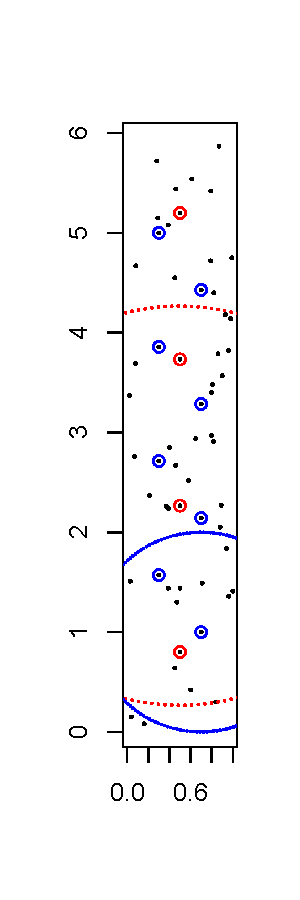
\includegraphics[width=\linewidth]{../simulation/plots/nodes_2_108}
\caption{}
\label{fig: nodes locations, case 2}
\end{subfigure}
\end{minipage}
\begin{minipage}{.79\textwidth}
\begin{subfigure}{\textwidth}
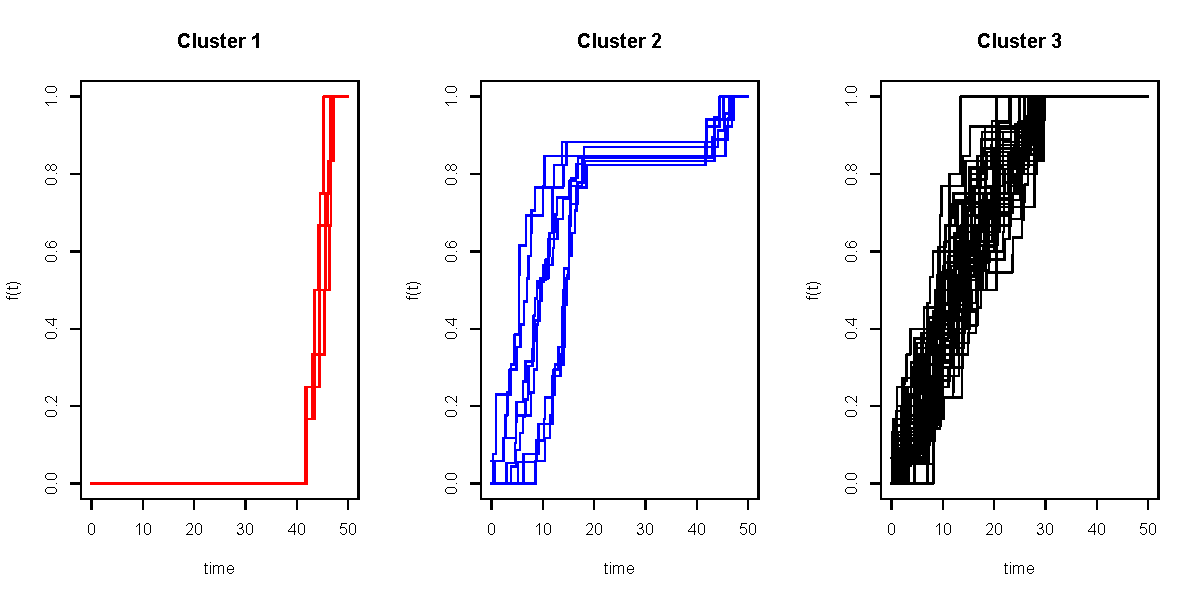
\includegraphics[width=\linewidth]{../simulation/plots/f_list_2_108}
\caption{}
\label{fig: original curves, case 2}
\end{subfigure}
\begin{subfigure}{\textwidth}
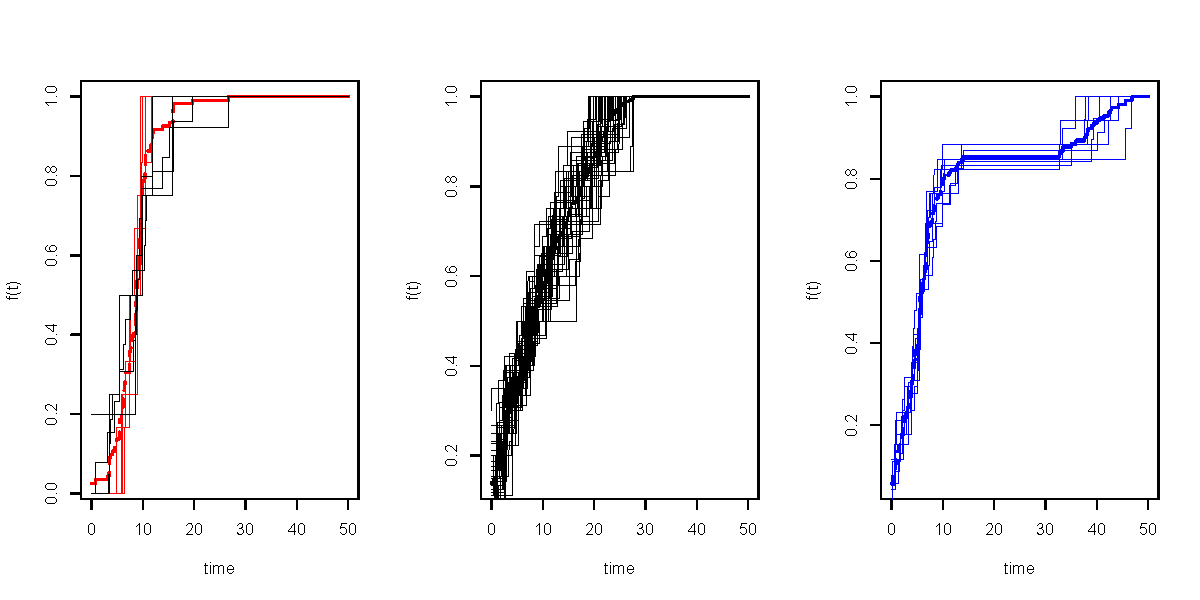
\includegraphics[width=\linewidth]{../simulation/plots/clus_results_2_108}
\caption{}
\label{fig: aligned curves, case 2}
\end{subfigure}
\end{minipage}
\caption{(a): Locations of nodes. Each black dot represents a node, the four type I nodes are marked as red, and eight type II nodes are marked as blue. The dotted red and blue circles explain the reachable area of the type I node and type II node, respectively. (b): Original empirical distribution functions. The red, blue and black curves correspond to type I, II, III nodes, respectively. (c): Clustering result. Each subplot includes the shifted distribution functions of nodes belonging to that cluster. The mean curves are plotted by dashed lines. }
\end{figure}
Another case with three clusters is also tested. 
The locations of nodes are displayed in Figure \ref{fig: nodes locations, case 2}.
The connecting radius for type I node is set as $2$, and that for other nodes is set as $1$. 
For a pair of type III nodes, the connecting time is generated from uniform distribution $U(0,30)$.
For the pair of nodes with one from type II and the other from type III, 
the connecting time is distributed as $N(5+\tau,4)$, where $\tau$ is the time delay caused by the type II node and is generated randomly from $U(0,10)$.
For the pair of nodes with one from type I and the other from type II, the connecting time is distributed as $U(\tau,\tau+6)$, where $\tau$ is the time delay caused by the type II node and is generated randomly from $U(40,42)$.
\\
Figure \ref{fig: original curves, case 2} shows the empirical distribution function of the connecting time of each node. Due to the time delay of type I node, the distribution function of type II nodes are not identically distributed anymore.
Figure \ref{fig: aligned curves, case 2} shows clustering result. All nodes except four type III node are clustered correctly.
\\
10 independent trials are recorded. 
The k-means++ initialization is applied for each trial.
Among the ten trials, the number of incorrectly clustered nodes is $2.6\pm 3.37$.

 

[Will add another case where the algorithm fails.]

% To show the development of the network, we plot snapshots in Fig.\ref{Fig: development of network} of the network $\mathbf{G}_1$  at time points $t=0.01, 0.1, 1, 10, 100$.
% \begin{figure}
% \centering
% 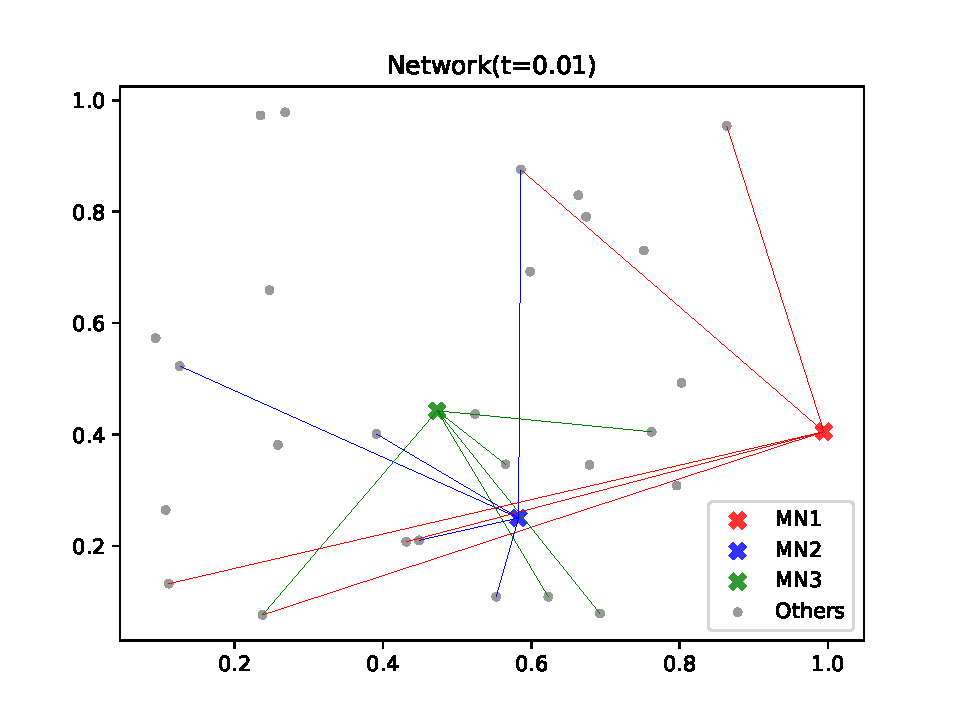
\includegraphics[width = 0.3\textwidth]{Graphs/t_001.pdf}
% 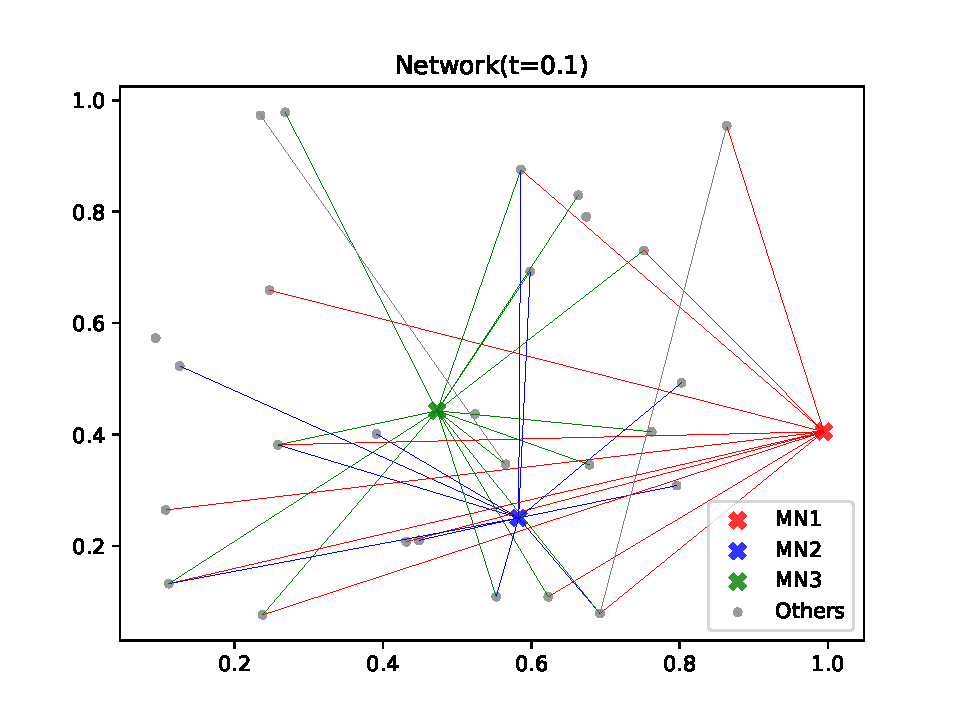
\includegraphics[width = 0.3\textwidth]{Graphs/t_01.pdf}
% 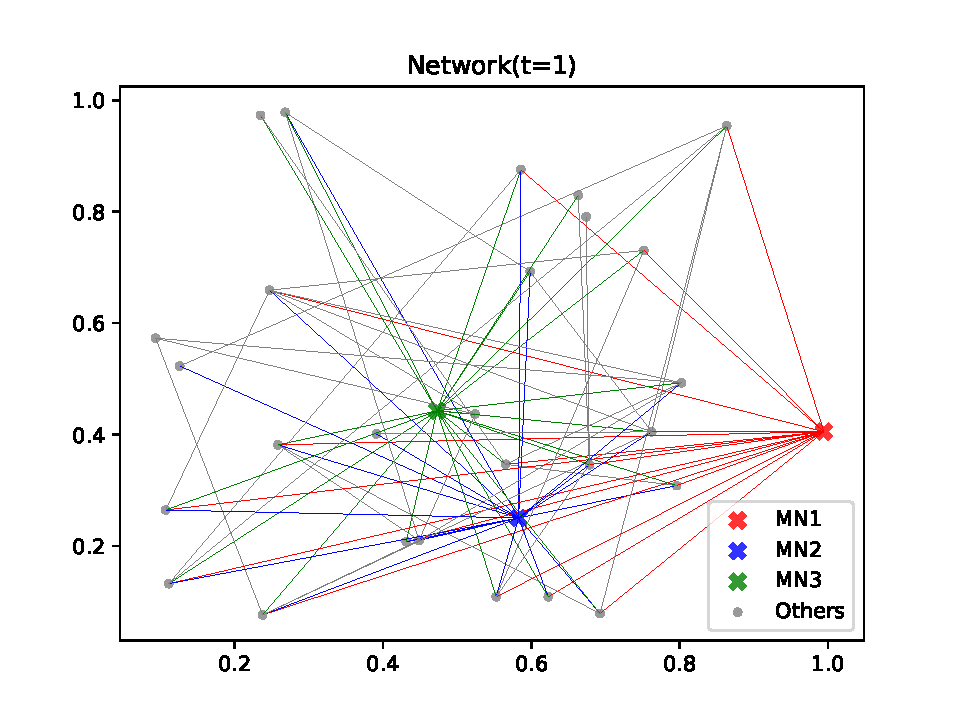
\includegraphics[width = 0.3\textwidth]{Graphs/t_1.pdf}\\
% 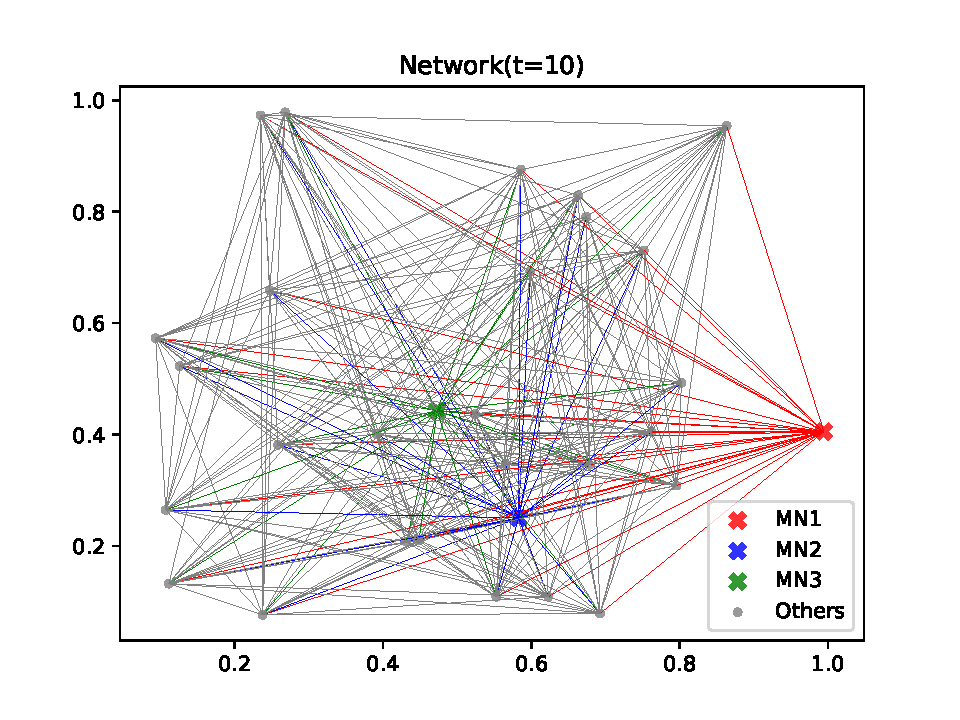
\includegraphics[width = 0.3\textwidth]{Graphs/t_10.pdf}
% 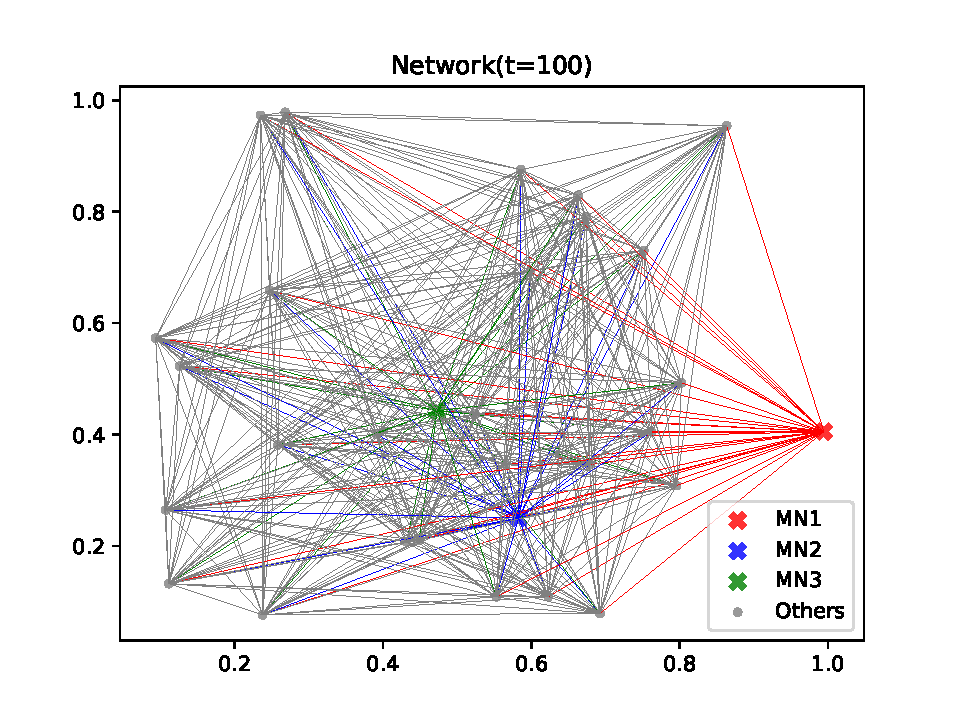
\includegraphics[width = 0.3\textwidth]{Graphs/t_100.pdf}
% \caption{Development of the network with two cell types. The node $n_1$ is represented by ``MN1'' in red. The node $n_2$ is represented by ``MN2'' in blue. The node $n_3$ is represented by ``MN3'' in green. Other nodes are represented by ``Others'' in gray.}
% \label{Fig: development of network}
% \end{figure}


